\chapter{Intro}
\label{ch:Intro}

In diesem Abschnitt wird zunächst das Projekt \textbf{OpenSourceStats} allgemein vorgestellt und Zweck sowie Funktionalität erläutert.
Damit soll ein generelles Verständnis des Projekts geschaffen werden, sodass Erläuterungen in späteren Abschnitten nachvollziehbar sind.
\subsection*{Zweck des Projekts}
Ziel des Projekts ist die Entwicklung einer Android-App, die es ermöglichen soll, Statistiken über GitHub-Contributions anzuzeigen.
Als Contribution versteht GitHub Commits, Issues, Pull-Requests und Pull-Request-Reviews.
Die Bezeichnungen in der App sollen dabei den Bezeichnungen der offiziellen API folgen (siehe \href{https://docs.github.com/en/graphql/reference/objects#contributionscollection}{API-Dokumentation}).
Damit soll diese App eine Funktion erfüllen, die in der offizielle GitHub-App (noch) nicht implementiert ist.
\subsection*{Funktionen}
Die App soll verschiedene Funktionen anbieten, die auf mehrere Unterseiten des User-Interfaces verteilt sein sollen.
Als Hauptfunktion soll die App ein Dashboard bereitstellen, dass eine schnelle und übersichtliche Zusammenfassung der letzten Contributions anzeigt.
Dabei werden die Contributions nach Wochen oder Monaten gruppiert.
Tatsächlich angezeigt werden die Daten der aktuellen und letzten Woche, sowie des aktuellen und letzten Monats.
Außerdem sollen im Dashboard die Tage mit den meisten Contributions und meisten Commits angezeigt werden.
Abbildung \ref{fig:dashboard_screenshot} zeigt beispielhaft, wie die App diese Daten anzeigt.

\begin{figure}
    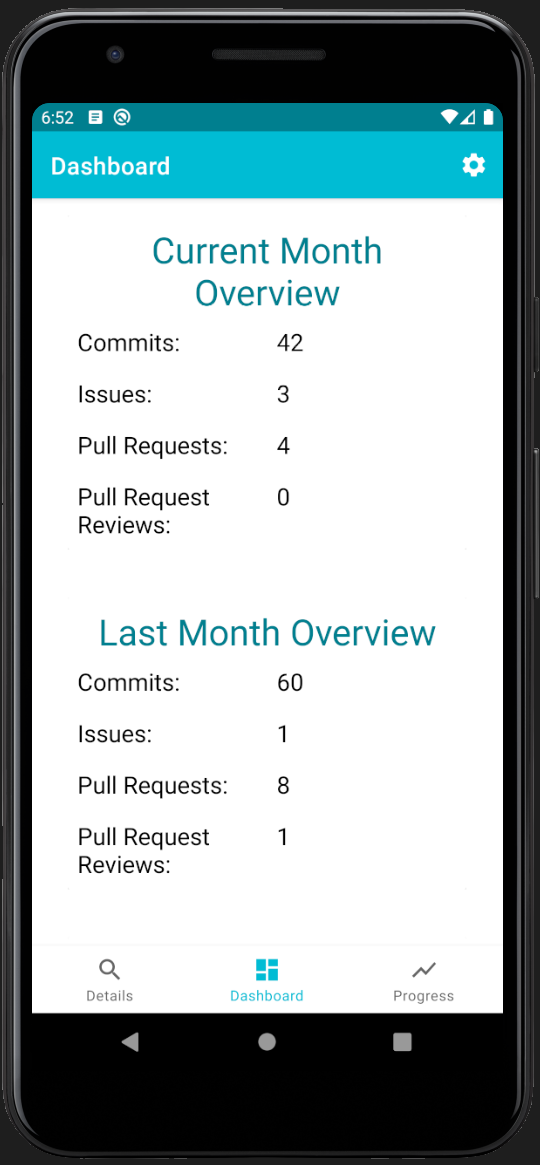
\includegraphics[height=10cm]{screenshot_dashboard.png}
    \centering
    \caption{Screenshot des Dashboards}
    \label{fig:dashboard_screenshot}
\end{figure}
Eine weitere Funktion soll sein, die Veränderung der Contributions in definierten Zeiträumen zu berechnen und anzuzeigen.
Dafür soll eine eigene Unterseite mit dem Titel "Progress" bereitgestellt werden.
Die Prozentuale Veränderung soll auf Wochen und Monatsbasis angezeigt werden, wie auch in Abbildung \ref{fig:progress_screenshot} gezeigt.

\begin{figure}
    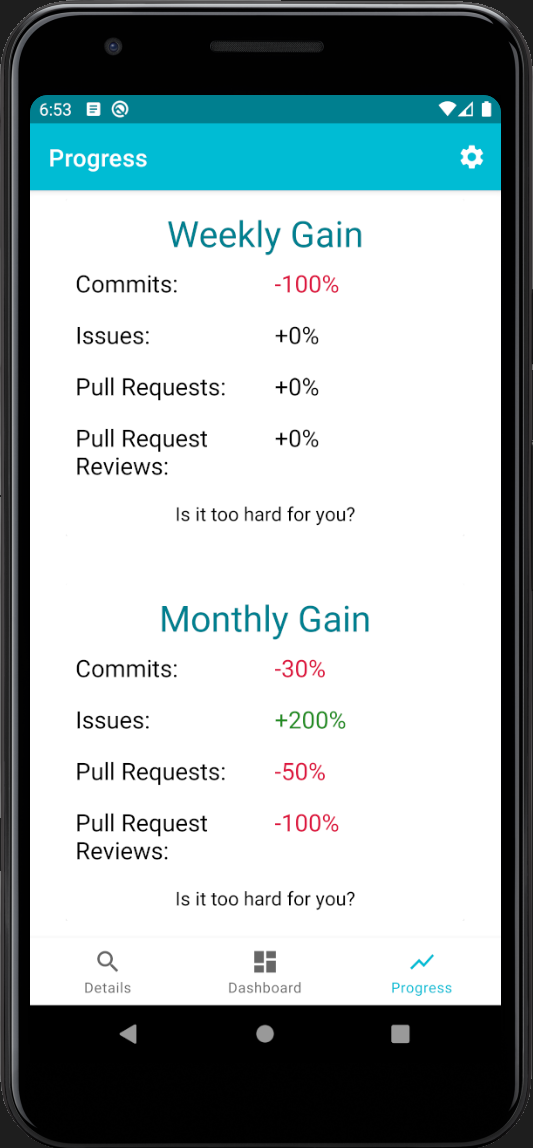
\includegraphics[height=10cm]{screenshot_progress.png}
    \centering
    \caption{Screenshot der Progress-Ansicht}
    \label{fig:progress_screenshot}
\end{figure}
Weiterhin soll es eine Details-Unterseite geben, die es erlaubt, Details über die Repositories anzuzeigen, zu denen die Contributions zugeorndet sind.
Dabei soll es möglich sein, nach Art der Contribution zu differenzieren.
Das bedeutet, dass es zum Beispiel die Möglichkeit gibt, nur Repositories mit Commits anzuzeigen.
Abbildung \ref{fig:repository_details_screenshot} zeigt beispielhaft, die Anzeige von Beschreibung, Erstelldatum und Programmiersprachen eines Repository.
Weiterhin soll das System hier dem Nutzer erlauben beliebige Zeiträume für die Auswertung auszuwählen.

\begin{figure}
    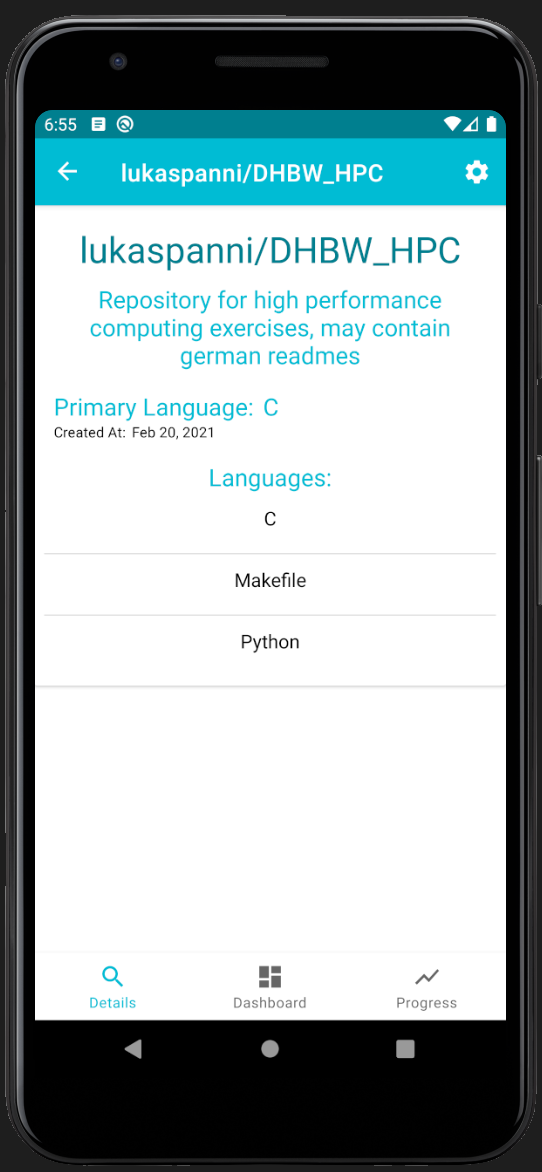
\includegraphics[height=12cm]{screenshot_repository_details.png}
    \centering
    \caption{Screenshot der Repository-Details}
    \label{fig:repositry_details_screenshot}
\end{figure}
Um diese Funktionen umzusetzen soll die GitHub-API verwendet werden.
Dafür ist eine Authentifizierung mit dem GitHub-Account des Nutzers mit Hilfe des OAuth-Protokolls notwendig.
Für eine möglichst gute User-Experience sollen die Daten nicht immer über die API abgerufen werden, sondern in einem lokalen Cache für eine definierte Zeit vorgehalten werden.
Wenn die Daten nicht aus dem lokalen Cache geladen werden können sollen die Daten asynchron über die API abgerufen werden.
Die Asyncrhone Kommunikation dient ebenfalls dazu, die User-Experience zu verbessern.